\section{Anforderungsspezifikation}
\label{sec:Anforderungsspezifikation}

\subsection{Use Cases}
\label{sub:Use Cases}
Im folgenden sind die funktionalen Anforderungen an PlazaRoute mit all seinen Komponenten, welche im Kapitel \ref{sec:Architektur} aufgeführt sind, als Use Cases im Brief-Format beschrieben. Zur Übersicht folgt zuerst das Use Case Diagramm in Abbildung \ref{fig:usecase_diagram}.

\begin{figure}[ht]
\centering
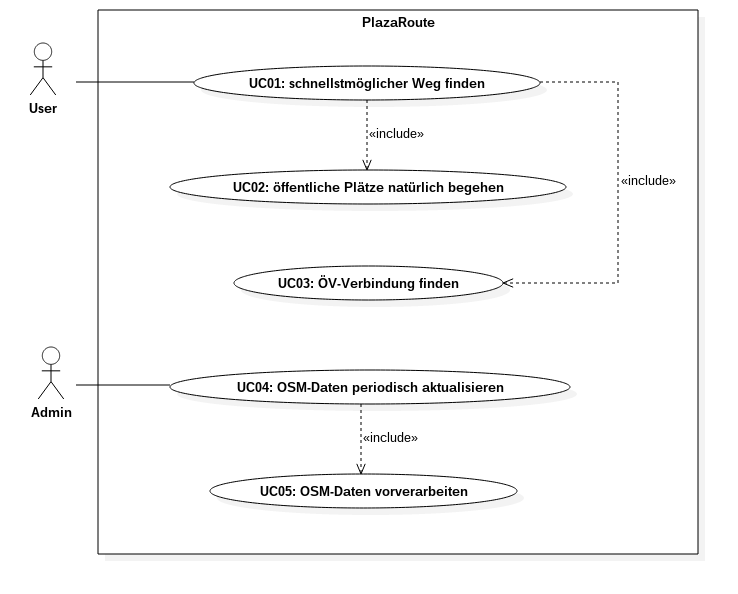
\includegraphics[width=1\linewidth]{projectdoc/img/usecase_diagram}
\caption[Use Case Diagramm]{Use Case Diagramm}
\label{fig:usecase_diagram}
\end{figure}

\subsubsection{Aktoren}
\label{uc:Aktoren}

\begin{table}[h]
    \centering
    \caption{Aktoren}
    \label{aktoren}
    \begin{tabular}{ll}
        \textbf{Aktor} & \textbf{Beschreibung und Interessen}                                                                                                                                                                                     \\
        \textbf{User}  & \begin{tabular}[c]{@{}l@{}}Ein User ist ein Fussgänger, welcher schnellstmöglich von Punkt A zu Punkt B kommen möchte. \\ Er fungiert in der Komponente QGIS-Plugin.\end{tabular}                                          \\
        \textbf{Admin} & \begin{tabular}[c]{@{}l@{}}Ein Admin ist daran interessiert, dass aktuelle Daten dem Aktor User zur Verfügung stehen. \\ So möchte er Daten vorverarbeiten und dem Aktor User zur Verfügung stellen können.\end{tabular}
    \end{tabular}
\end{table}

\subsubsection{UC01: schnellstmöglicher Weg finden}
\label{usecase:UC01}
Aktoren: \emph{User}

Nachdem der User einen Start- und Endpunkt (geografische Standorte) bekannt gegeben hat, erhält er den schnellstmöglichen Weg, welcher mit öffentlichen Verkehrsmitteln und zu Fuss machbar ist.
Dabei soll die maximale Laufdistanz zur ersten Haltestelle nicht mehr als 2km betragen.


\subsubsection{UC02: kürzester Pfad über öffentliche Plätze nehmen}
\label{usecase:UC02}
Aktoren: \emph{User}

Der Fussgänger möchte während dem Laufen, nicht um Plätze herumgeroutet werden, sondern den kürzesten Weg über den öffentlichen Platz nehmen.

\subsubsection{UC03: öffentliche Plätze natürlich begehen}
\label{usecase:UC03}
Aktoren: \emph{User}

Als Fussgänger möchte ich öffentliche Plätze natürlich (Verweis auf Definition Natürlichkeit) begehen.


\subsubsection{UC04: OSM-Daten periodisch aktualisieren}
\label{usecase:UC04}

Als Benutzer möchte ich auf den wöchentlich aktuellsten \ac{OSM}-Daten routen können.

\subsubsection{UC05: OSM-Daten vorverarbeiten}
\label{usecase:UC05}

\subsection{System-Sequenzdiagramme}
\label{sub:System-Sequenzdiagramme}

TODO

\subsection{Weitere Funktionen}
\label{sub:Weitere Funktionen}

TODO

\subsection{Nicht-funktionale Anforderungen}
\label{sub:Nicht-funktionale Anforderungen}

\subsubsection{NFA01: }
\label{NFA:NFA01}

PlazaRoute wird in ein oder mehreren Docker-Images ausgeliefert

\subsubsection{NFA02: austauschbare Routing-Engine}
\label{NFA:NFA02}

austauschbare Routing Engine

\subsubsection{NFA03: periodische Aktualisierung der OSM-Daten}
\label{NFA:NFA03}

Die auf Fussgänger optimierten Routing-Graphen werden wöchentlich mit den neuesten \ac{OSM}-Daten vorverarbeitet.

\subsubsection{NFA04: Dauer der Vorverarbeitung}
\label{NFA:NFA04}

Die Vorverarbeitung der \ac{OSM}-Daten (Optimierung auf öffentliche Fläche) darf maximal 1 Stunde benötigen

\subsubsection{NFA05: zusätzliche Datenmenge}
\label{NFA:NFA05}

Die zusätzlichen Daten für die Optimierung dürfen nicht mehr als x% des Kartenmaterials

\subsubsection{NFA06: Dauer des Unterbruchs bei OSM-Daten-Integration}
\label{NFA:NFA06}

Verfügbarkeit: Unterbruch des Services beim Integrieren der neuesten \ac{OSM}-Daten (für Router Neuberechnung) max. 2 Stunden

\subsection{Detailspezifikation}
\label{sub:Detailspezifikation}

TODO